\documentclass{csri10}

% PACKAGES ---------------------------------------------------------------
\usepackage{amsfonts,amsmath,graphicx,subfigure}
% ADD YOUR OWN PACKAGES HERE ---------------------------------------------
%\usepackage{someotherpackage}

% DEFINITIONS ------------------------------------------------------------
% ADD YOUR OWN DEFINITIONS HERE ------------------------------------------
% BE SURE TO PREFACE LABEL WITH YOUR OWN INITIALS (SSS in this example) --
\newcommand{\SSSnorm}[1]{\left\Vert#1\right\Vert}
\newcommand{\SSSabs}[1]{\left\vert#1\right\vert}

% This controls the table-of-contents entry in the proceedings. Edit it
% to include your article title followed by the authors' names, as shown.
\addcontentsline{toc}{chapter}{Optika: A GUI Framework for Parameterized Applications\\
{\em Kurtis Nusbaum Student and Dr.\ Mike Heroux Mentor}}

\pagestyle{myheadings}

\thispagestyle{plain}

% This gives the running head. Usually you list a shortened version of
% your article title (unless it's already very short) along with
% the author's names, as shown.
\markboth{Optika GUI Framework}{Kurtis Nusbaum Student and Dr.\ Mike Heroux Mentor}

% Put your article title in here
\title{Optika: A GUI Framework for Parameterized Applications}

% List each author, their affiliation, and their e-mail address, as shown.
\author{Kurtis L.\ Nusbaum\thanks{St. John's University, klnusbaum@csbsju.edu} \and Dr.\ Mike Heroux\thanks{Sandia National Laboratories,
maherou@sandia.gov}}

\begin{document}

\maketitle

% Include your abstract here.
\begin{abstract}
In the field of scientific computing there are many specialized programs designed for specific applications 
in areas like biology, chemistry, and physics. These applications are often very powerful and extraodinarily 
useful in their respective domains. However, many suffer from a common problem: a poor user interface. Many 
of these programs are homegrown, and the concern of the designer was not ease of use but rather 
functionality. The purpose of Optika is to address this problem and provide a simple, viable solution. Using
only a list of parameters passed to it, Optika can dynamically generate a GUI. This allows the user to specify 
parameters values in fashion that is much more intuitive than the traditional "input decks" used by many 
parameterized scientific applications. By leverageing the power of Optika, these scientific applications 
will become more accessible and thus allow their designers to reach a much wider audience while requiring 
minimal extra development effort.

\end{abstract}

\section{Introduction} \label{SSS:sec:intro}
I like chocolate pudding.  For that matter everyone else does too. This relationship is captured in \eqref{SSS:eq:one},
\begin{equation}\label{SSS:eq:one}
f(x) = x^{100-d},
\end{equation}
where $f$ is happiness in utils, $x$ is the quantity of chocolate pudding consumed in ounces and $d$ is the age of the
subject in years.

It has been argued that that chocolate pudding consumption by age is shown in Figure \ref{SSS:fig:Mentor05}.  However,
we propose an alternative pudding consumption model, shown in Figure \ref{SSS:fig:cos}.

\begin{figure}[hbh]
\begin{center}
\scalebox{0.5}{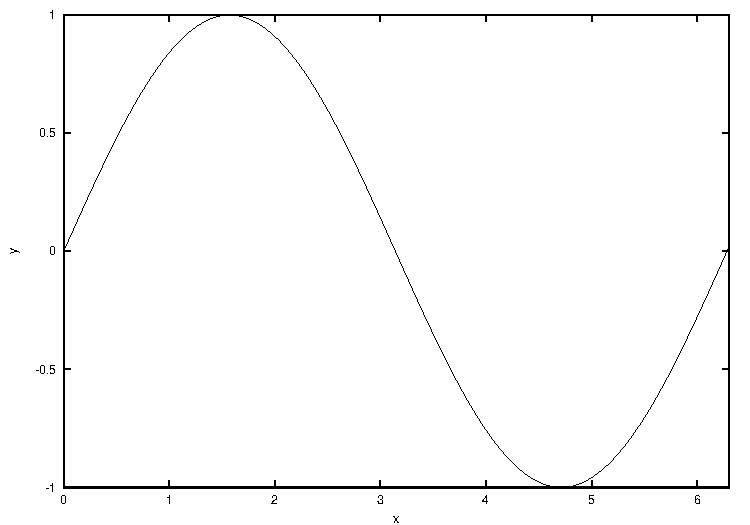
\includegraphics{plots/sinx}} \caption{Chocolate pudding consumption model of
\cite{SSS:Mentor05}}\label{SSS:fig:Mentor05}
\end{center}\end{figure}

\begin{figure}[htb]
\begin{center}
\scalebox{0.5}{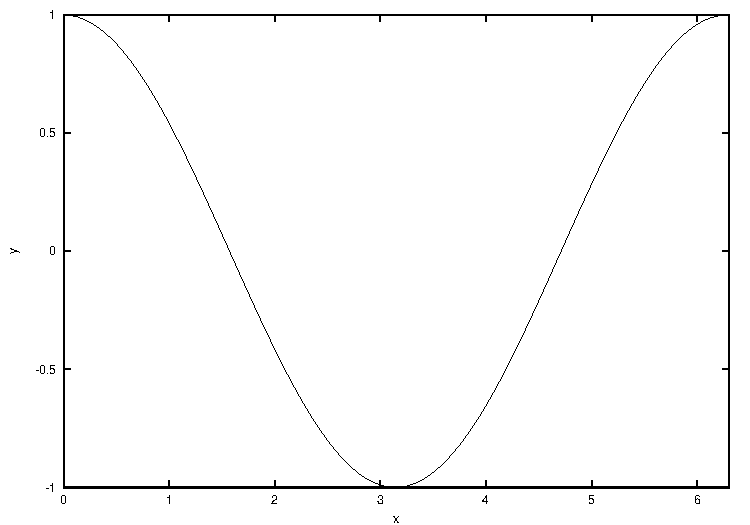
\includegraphics{plots/cosx}} \caption{Proposed chocolate pudding consumption model}\label{SSS:fig:cos}
\end{center}\end{figure}

We also want to show these figures side by side, to better illustrate our comparison.  We can see this in Figures
\ref{SSS:fig:comp1} and \ref{SSS:fig:comp2}.

\begin{figure}[htb]
\begin{center}
\subfigure[M. Mentor's Model]{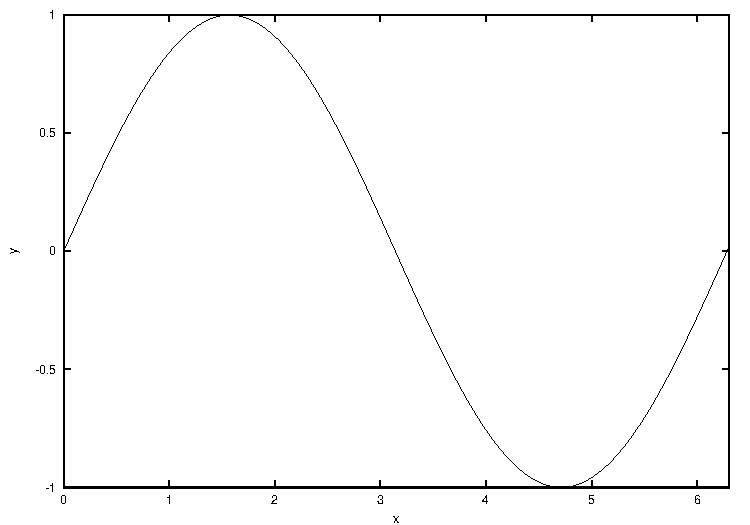
\includegraphics[scale=.5]{plots/sinx}\label{SSS:fig:comp1}} \subfigure[Proposed
Model]{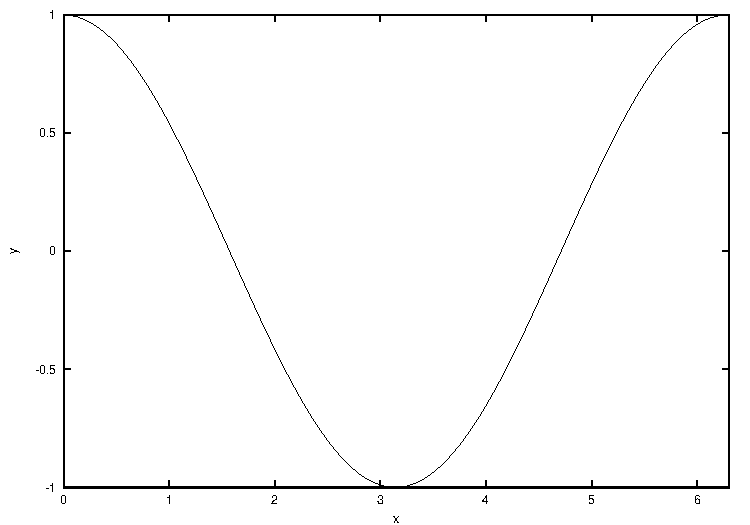
\includegraphics[scale=.5]{plots/cosx}\label{SSS:fig:comp2}} \caption{Comparative chocolate pudding consumption
models}
\end{center}\end{figure}

\section{Actual Content}

As we saw in Section \ref{SSS:sec:intro}, we all like chocolate pudding. This is where I wish
\textsf{$\setminus$jargonfill} worked. It would fill the page with meaningless technobabble so I could illustrate this
package. Instead, I'll talk about how to use quotations in latex. "Never use these quotations." ``Always use these,
instead.''

\section{Conclusions}
Herein, we repeat the abstract in past tense.

Unlike many other baked goods, chocolate pudding is subject to a myriad of interesting (and unique) effects on both the
meso and nano scales.  Understanding these phenomena is critical, not only to America's restaurant industry, but to
children everywhere.  We have examined these effects and have proposed new potential models which accurately capture
the material structure of chocolate pudding.

\bibliographystyle{siam}
% Edit the line below to be your first and last names.
\bibliography{FirstnameLastname}

% Edit FirstnameLastname below to be your first and last names, but leave the line commented out.
% This line will help me merge bibliographies for the proceedings.
%\input{FirstnameLastname/FirstnameLastname.bbl}

\end{document}
